\section{Programmable Storage}
\label{sec:progly}

When application requirements are not met by an underlying storage system the
most common approach is to design workarounds that roughly fall into one
of three categories:

{\bf Extra services.} ``Bolt-on'' services are intended to improve performance
or enable a feature, but come at the expense of additional hardware, software
sub-systems, and dependencies that must be managed, as well as trusted.
For instance, many extensions to Hadoop have been created to address its
limitations~\cite{bu:vldb2010-haloop, ekanayake:hpdc2010-twister,
ekanayake:escience2008-eglmapreduce, mihailescu:hotstorage2012-mixapart}.

{\bf Application changes.} The second approach to adapting to a storage system
deficiency is to change the application itself by adding more data management
intelligence into the application or as domain-specific middleware. When
application changes depend on non-standard semantics exposed by the storage
system (e.g., relaxed POSIX file I/O or MPI-IO hints), the coupling that results
can be fragile.
For example, SchiHadoop~\cite{buck:hpc2011-scihadoop} and Rhea~\cite{gkantsidis:nsdi2013-rhea} both do
an excellent jobs of partitioning data in Hadoop applications, but may not
stand the test of time for future workloads, since the partitioning is
specific to scientific data.

{\bf Storage modifications.} When these two approaches fail to meet an
application's needs, developers may turn their attention to any number of
heavyweight solutions ranging from changing the storage system itself, up to
and including designing entirely new systems. This approach can require
significant cost, domain knowledge, and extreme care when building or
modifying critical software that can take years of code-hardening to trust.
For example, HDFS fails to meet many needs 
of metadata-intensive workloads~\cite{shvachko:login2012-hdfs-scalability}.
This has lead to modifications to its architecture or
API~\cite{balmin:sigmod2012-clydesdale} to improve performance.

Rather than relying on storage systems to evolve \emph{or} applications to
change, a hybrid approach that embraces interface instability without placing
an unmanageable burden on developers is ``The Malacology Approach".

\subsection{The Malacology Approach}

%\textcolor{red}{HELP! We can't decide if this section should be called ``The
%Programmable Storage Approach" or ``The Malacology Approach" -- I argue that
%Malacology is the prototype but Noah thinks Malacology Approach makes more
%sense.}

A programmable storage system helps future programmers co-design applications
and storage systems by exposing existing internal services so that 
they can be composed to form application specific
services~\cite{sevilla:eurosys17}.
Figure~\ref{fig:malacology} shows the architecture of Malacology, a prototype programmable storage system
implemented in Ceph, which exposes a variety of low-level internal services
such as custom object interfaces, cluster metadata management, and
load-balancing. While Ceph natively exposes file, block, and object
abstractions, Malacology demonstrated the construction of two real-world
services (ZLog~\cite{watkins:ucsc-soe-16-12} and Mantle~\cite{sevilla:sc15-mantle}) using only the composition of existing interfaces present in Ceph.

\begin{figure}[t]
\centering
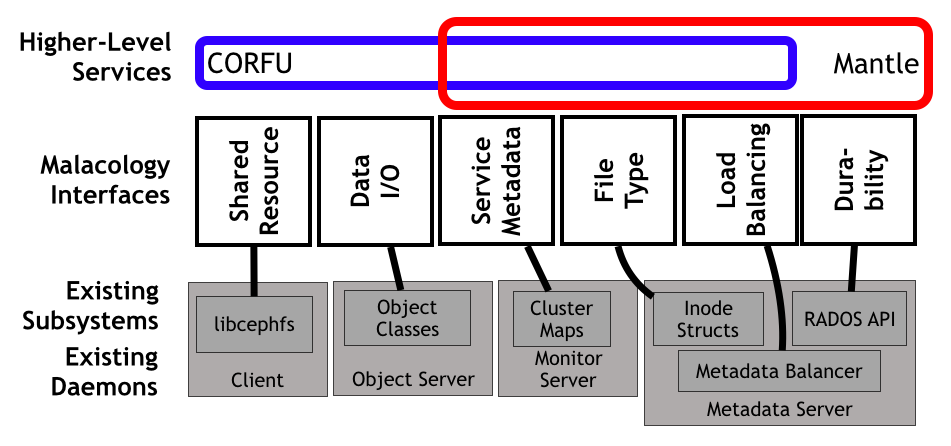
\includegraphics[width=1.0\linewidth]{implementation-overview.png}
\caption{Malacology implementation in Ceph. Existing sub-systems are composed
    to form new services and application-specific optimizations.}
\label{fig:malacology}
\end{figure}

ZLog is a high-performance distributed shared
log that implements the CORFU protocol~\cite{balakrishnan:nsdi12}.
This protocol achieves high-throughput using a soft-state network-attached
counter, and stripes log content over a cluster of flash devices each with a
protocol-specific storage interface. While CORFU is a stand-alone system,
Malacology is able to instantiate the same abstraction and approximate 
the same unique optimizations.

Malacology reproduces the CORFU network-attached counter service using a
capability-based mechanism found in the Ceph distributed file system for
managing cached metadata. ZLog implements the counter using the metadata server's ability to provide temporary
exclusive access to a shared resource (in this case, file metadata).  In ZLog, CORFU's storage device interface is
constructed using application-specific object interfaces in Ceph. These
software-based interfaces are constructed as a composition of low-level I/O
interfaces (e.g. an LSM-tree and a bytestream) that operate in an atomic
context allowing the interface to maintain consistency across native
interfaces.

The demonstration of interface synthesis in Malacology suggests a new form of
application development that significantly reduces the number of lines of code.
While this ability to construct software-defined interfaces is powerful,
next we will show how access to low-level interfaces can be a double-edged
sword, which provides power at the cost of increased maintenance complexity.
